\emph{Valoració}

La practica ha resultat molt interessant, al principi va costar un poc adequar l'entorn de treball.
Per tal de poder emprar la llibreria i el simulador \emph{MobileSim} en la Debian que empram normalment
va requerir compilar-ho de nou cosa que generà algun problema de dependències però va quedar sobradament
compensat per la comoditat de no haver de emprar una màquina virtual.

Cal destacar que el Mapper3Basic i el MobileSim son de gran ajuda a l'alumne i permeten fer simulacions
per res comparables amb la primera pràctica del braç robot.

La llibreia Aria en general esta força be i es bastant intuïtiva, rara vegada s'ha hagut de cercar
informació addicional que no figurés a la API.

Per altra banda s'ha de mencionar que el C++ ens ha suposat algun mal de cap, sobretot en l'ambit
de visibilitat dels procediments i l'ús de punters. En aquest sentit ens hagués agradat tenir temps
per provar de fer la practica amb \emph{Python}, l'únic fet que ens tirà enderrere es que no sabiem si funcionaria
el simulador i que possiblement la llibreria no està insta\lgem al robot real.

També ens han portat molts mal de cap el trobar valors adequats per cada una de les ponderacions i llindars,
sovint ens trobavem que amb certa combinació de llindars, especialment als de heading el robot podia quedar
fent voltes sobre si mateix si el punt on havia d'anar era proper al punt actual pero havia de fer un canvi
d'orientació.

\begin{figure}[H]
\begin{center}\label{headingthproblem}
 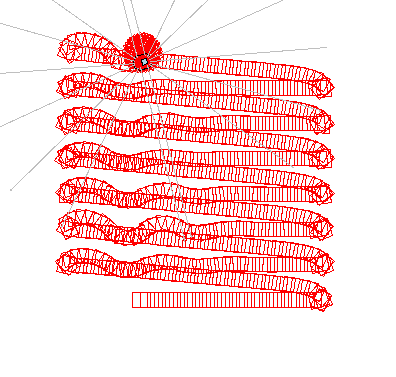
\includegraphics[width=0.7\textwidth]{diagrames/figures/voltes.png}
 % ordreRotacions.png: 1286x768 pixel, 150dpi, 21.77x13.00 cm, bb=0 0 617 369
\end{center}
  \caption{Problema amb llindar de heading}
\end{figure}

Atribuirem aquest problema a que el robot inicia el moviment abans d'estar orientat pero donat que la
proximitat es molt gran no acaba d'orientar-se mai.

Tot i així i encara que nes hagues agradat implementar alguna cosa més consideram la pràctica acabada
i assolits els coneixements bàsics assolits i que per tant les implementacions que tenim en ment
es converteien en rutina ja que no requereixen conceptes nous sino simples combinacions dels ja implementats.